% Figure 7: Baseline Comparison (replaces subjective bar chart)
\documentclass[tikz,border=5pt]{standalone}
\usepackage{pgfplots}
\pgfplotsset{compat=1.18}

\begin{document}
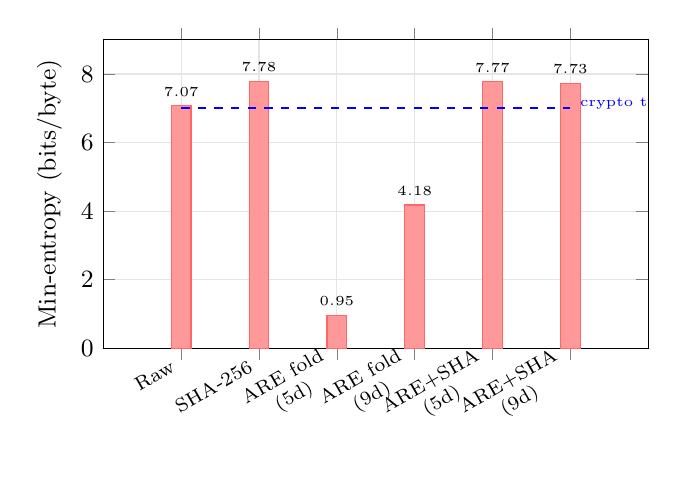
\begin{tikzpicture}
\begin{axis}[
  width=8.5cm, height=5.5cm,
  ybar,
  bar width=0.25cm,
  enlarge x limits=0.2,
  ylabel={Min-entropy (bits/byte)},
  symbolic x coords={Raw, SHA-256, {ARE fold\\(5d)}, {ARE fold\\(9d)}, {ARE+SHA\\(5d)}, {ARE+SHA\\(9d)}},
  xtick=data,
  x tick label style={rotate=30, anchor=east, font=\scriptsize, align=center},
  ymin=0, ymax=9,
  ytick={0,2,4,6,8},
  grid=major,
  grid style={gray!20},
  font=\small,
  nodes near coords,
  nodes near coords style={font=\tiny, above},
  every node near coord/.append style={rotate=0},
]

\addplot[fill=red!40, draw=red!60] coordinates {
  (Raw, 7.07)
  (SHA-256, 7.78)
  ({ARE fold\\(5d)}, 0.95)
  ({ARE fold\\(9d)}, 4.18)
  ({ARE+SHA\\(5d)}, 7.77)
  ({ARE+SHA\\(9d)}, 7.73)
};

% Threshold line
\draw[dashed, thick, blue] (axis cs:Raw, 7.0) -- (axis cs:{ARE+SHA\\(9d)}, 7.0);
\node[font=\tiny, blue, anchor=west] at (axis cs:{ARE+SHA\\(9d)}, 7.15) {crypto threshold};

\end{axis}
\end{tikzpicture}
\end{document}
